%%****************************************************************************
%** Copyright 2002, 2003 by Lukas Ruf, <ruf@topsy.net>
%** Information is provided under the terms of the
%** GNU Free Documentation License <http://www.gnu.org/copyleft/fdl.html>
%** Fairness: Cite the source of information, visit <http://www.topsy.net>
%****************************************************************************
%** Last Modification: 2005-07-11 1600
%** 2005-07-11	Bernhard Tellenbach
%**							Switched default document class to: book
%**							Added \include{appendix.tex}
%****************************************************************************

%\documentclass[10pt,final,a4paper,twoside]{book}
%\documentclass[10pt,draft,a4paper,oneside]{report}
\documentclass[headings=optiontohead,10pt,final,a4paper,oneside]{scrreprt}
%\documentclass[10pt,draft,a4paper,oneside]{article}

%**Latex Master Document*********

%** preamble.tex: here all the document-wide settings
%                 are defined
\RequirePackage{times}

%\usepackage[english]{babel}
%-% \usepackage[german]{babel}
\usepackage[ngerman]{babel}

\usepackage[utf8]{inputenc}
\usepackage[T1]{fontenc}
\usepackage{textcomp}
\usepackage{type1cm}
\usepackage[table,xcdraw]{xcolor}
\usepackage{a4}

\usepackage{graphicx}
\graphicspath{{Figures/},{Pictures/}}
\usepackage{subfigure}

\usepackage{fancyhdr}
\usepackage{fancybox}
\usepackage{hyperref}

\usepackage{float}
\usepackage{longtable}
\usepackage{paralist}
\usepackage{url}
\usepackage{lscape}
\usepackage{moreverb}

\usepackage{makecell}
\usepackage{multirow}

\usepackage{tabularx}
\usepackage{xltabular}

\usepackage{nomencl}
  \let\abbrev\nomenclature
  \renewcommand{\nomname}{List of Abbrevations}
  \setlength{\nomlabelwidth}{.25\hsize}
  \renewcommand{\nomlabel}[1]{#1 \dotfill}
  \setlength{\nomitemsep}{-\parsep}
  %For old nomencl package, uncomment this:
  \makeglossary 
  %For new nomencl package, uncomment this:
  %\makenomenclature

\usepackage[normalem]{ulem}
  \newcommand{\markup}[1]{\uline{#1}}
  
   
\usepackage{ae,aecompl}


\usepackage[first,bottomafter,light]{draftcopy}
\draftcopyName{Draft v0.1}{120}

\addtolength{\textwidth}{2cm}
\addtolength{\textheight}{2cm}
\addtolength{\oddsidemargin}{-1.0cm}
\addtolength{\evensidemargin}{-1.0cm}
\addtolength{\topmargin}{-1.5cm}

%% No Serifs: Put comment markers in front of the next three lines otherwise
\renewcommand{\ttdefault}{cmtt}
\renewcommand{\rmdefault}{phv}  % Helvetica for roman type as well as sf
\renewcommand{\ttdefault}{pcr}  % use Courier for fixed pitch, if needed

\newcommand{\?}{\discretionary{/}{}{/}}
\newcommand{\liter}[0]{/home/ruf/Lib/Bibl/}
\newcommand{\fref}[1]{\mbox{Figure~\ref{#1}}}

\pagestyle{fancy}
%%-lpr Note: 'chapters' are defined for 'book's only
%%-lpr       in articles, we make use of sections only
\renewcommand{\chaptermark}[1]{\markboth{#1}{}}
\renewcommand{\sectionmark}[1]{\markright{\thesection\ #1}}
\fancyhf{}

%\fancyhead[LE,RO]{\bfseries\thepage}
%\fancyhead[LO]{\bfseries\rightmark}
%\fancyhead[RE]{\bfseries\leftmark}
\fancyhead[R]{\leftmark}
\fancyhead[L]{\rightmark}
\fancyfoot[R]{\thepage}
\fancyfoot[C]{ZHAW SoE}
\fancyfoot[L]{Bachelor Thesis (Informatik)}

\renewcommand{\headrulewidth}{0.5pt}
\renewcommand{\footrulewidth}{0.5pt}
\addtolength{\headheight}{0.5pt}
\fancypagestyle{plain}{%
   \fancyhf{}
   \fancyfoot[C]{\bfseries \thepage}
   \fancyhead{}%get rid of headers on plain pages
   \renewcommand{\headrulewidth}{0pt} % an the line
}
\newcommand{\clearemptydoublepage}{\newpage{\pagestyle{empty}\cleardoublepage}}

\setlength{\parindent}{0in}



\hyphenation{Strea-men}
\hyphenation{Apps}
\hyphenation{Threat}
\hyphenation{Init}

\newcommand{\Appendix}[2][?]
{
  \refstepcounter{section}
  \addcontentsline{toc}{appendix}
  {
    \protect\numberline{\appendixname~\thesection} %1
  }
  {
    \flushright\large\bfseries\appendixname\ \thesection\par
    \nohypens\centering#1\par
  }
  \vspace{\baselineskip}
}

\let\margin\marginpar
\newcommand\myMargin[1]{\margin{\raggedright\scriptsize #1}}
\renewcommand{\marginpar}[1]{\myMargin{#1}}

\newcommand\CHECK{\myMargin{CHECK}}
\newcommand\NEW{\myMargin{NEW}}

\usepackage[acronym,numberedsection=autolabel,section=section]{glossaries}

\makeglossaries

% \newacronym{<id>}{<short>}{<long>}

%\newglossaryentry{glos:mpegts}{
% name=MPEG Transport Stream,
% description={Von der Moving Picture Experts Group entwickeltes Transportstream-Protokoll für Video/Audio-Übertragung}
%}

\newacronym{ISP}{ISP}{Internet Service Provider}
\newacronym{OSS}{OSS}{Operations Support System}
\newacronym{NMS}{NMS}{Network Management System}
\newacronym{BSS}{BSS}{Business Support System}
\newacronym{CPE}{CPE}{customer premises equipment}
\newacronym{ADSL}{ADSL}{asymmetric digital subscriber line}
\newacronym{DSL}{DSL}{digital subscriber line}
\newacronym{VDSL}{VDSL}{very high-speed digital subscriber line}
\newacronym{PoP}{PoP}{point of presence}
\newacronym{B2B}{B2B}{business to business}
\newacronym{BGP}{BGP}{Border Gateway Protocol}
\newacronym{MPLS}{MPLS}{Multiprotocol Label Switching}
\newacronym{OSPF}{OSPF}{Open Shortest Path First}
\newacronym{FTTH}{FTTH}{Fiber To The Home}
\newacronym{FTTS}{FTTS}{Fiber To The Street}
\newacronym{OTO}{OTO}{Optical Telecommunication Outlet}
\newacronym{IRM}{IRM}{infrastructure resource modeling}

\newacronym{OMDF}{OMDF}{Optical Main Distribution Frame}
\newacronym{CLI}{CLI}{command line interface}

\newacronym{OHDF}{OHDF}{Optical Handover Distribution Frame}
\newacronym{IGP}{IGP}{Interior gateway protocol}

%% TODO: Definition Network Element

\newglossaryentry{glos:snmp}{
    name=Sinmple Network Management Protocol,
    description={}
}



\newglossaryentry{glos:isp}{
 name=MPEG Transport Stream,
 description={Von der Moving Picture Experts Group entwickeltes Transportstream-Protokoll für Video/Audio-Übertragung}
}


%\useshorthands*{"}
%\addto\extrasenglish{\languageshorthands{ngerman}}

\usepackage{csquotes}
\usepackage[
backend=biber,
bibstyle=ieee,
style=numeric,
sorting=none
]{biblatex}
\addbibresource{citations.bib}


\usepackage{pdfpages}
\usepackage{rotating}
\usepackage{pdflscape}

%% Adds another nesting level of numbering for sections
\setcounter{secnumdepth}{3}

\usepackage{helvet}
%\renewcommand*{\familydefault}{\sfdefault}

\usepackage{color,soul}

\usepackage[section,numbib,nottoc]{tocbibind}
\renewcommand{\listoffigures}{
    \tocsection
    \tocfile{\listfigurename}{lof}
}
\renewcommand{\listoftables}{
    \tocsection
    \tocfile{\listtablename}{lot}
}
% \newacronym{<id>}{<short>}{<long>}

%\newglossaryentry{glos:mpegts}{
% name=MPEG Transport Stream,
% description={Von der Moving Picture Experts Group entwickeltes Transportstream-Protokoll für Video/Audio-Übertragung}
%}

\newacronym{ISP}{ISP}{Internet Service Provider}
\newacronym{OSS}{OSS}{Operations Support System}
\newacronym{NMS}{NMS}{Network Management System}
\newacronym{BSS}{BSS}{Business Support System}
\newacronym{CPE}{CPE}{customer premises equipment}
\newacronym{ADSL}{ADSL}{asymmetric digital subscriber line}
\newacronym{DSL}{DSL}{digital subscriber line}
\newacronym{VDSL}{VDSL}{very high-speed digital subscriber line}
\newacronym{PoP}{PoP}{point of presence}
\newacronym{B2B}{B2B}{business to business}
\newacronym{BGP}{BGP}{Border Gateway Protocol}
\newacronym{MPLS}{MPLS}{Multiprotocol Label Switching}
\newacronym{OSPF}{OSPF}{Open Shortest Path First}
\newacronym{FTTH}{FTTH}{Fiber To The Home}
\newacronym{FTTS}{FTTS}{Fiber To The Street}
\newacronym{OTO}{OTO}{Optical Telecommunication Outlet}
\newacronym{IRM}{IRM}{infrastructure resource modeling}

\newacronym{OMDF}{OMDF}{Optical Main Distribution Frame}
\newacronym{CLI}{CLI}{command line interface}

\newacronym{OHDF}{OHDF}{Optical Handover Distribution Frame}
\newacronym{IGP}{IGP}{Interior gateway protocol}

%% TODO: Definition Network Element

\newglossaryentry{glos:snmp}{
    name=Sinmple Network Management Protocol,
    description={}
}



\newglossaryentry{glos:isp}{
 name=MPEG Transport Stream,
 description={Von der Moving Picture Experts Group entwickeltes Transportstream-Protokoll für Video/Audio-Übertragung}
}


%********************************

%** begin the document environment
\begin{document}

\frenchspacing
\sloppy

%** Titel.tex: Title page to be printed first

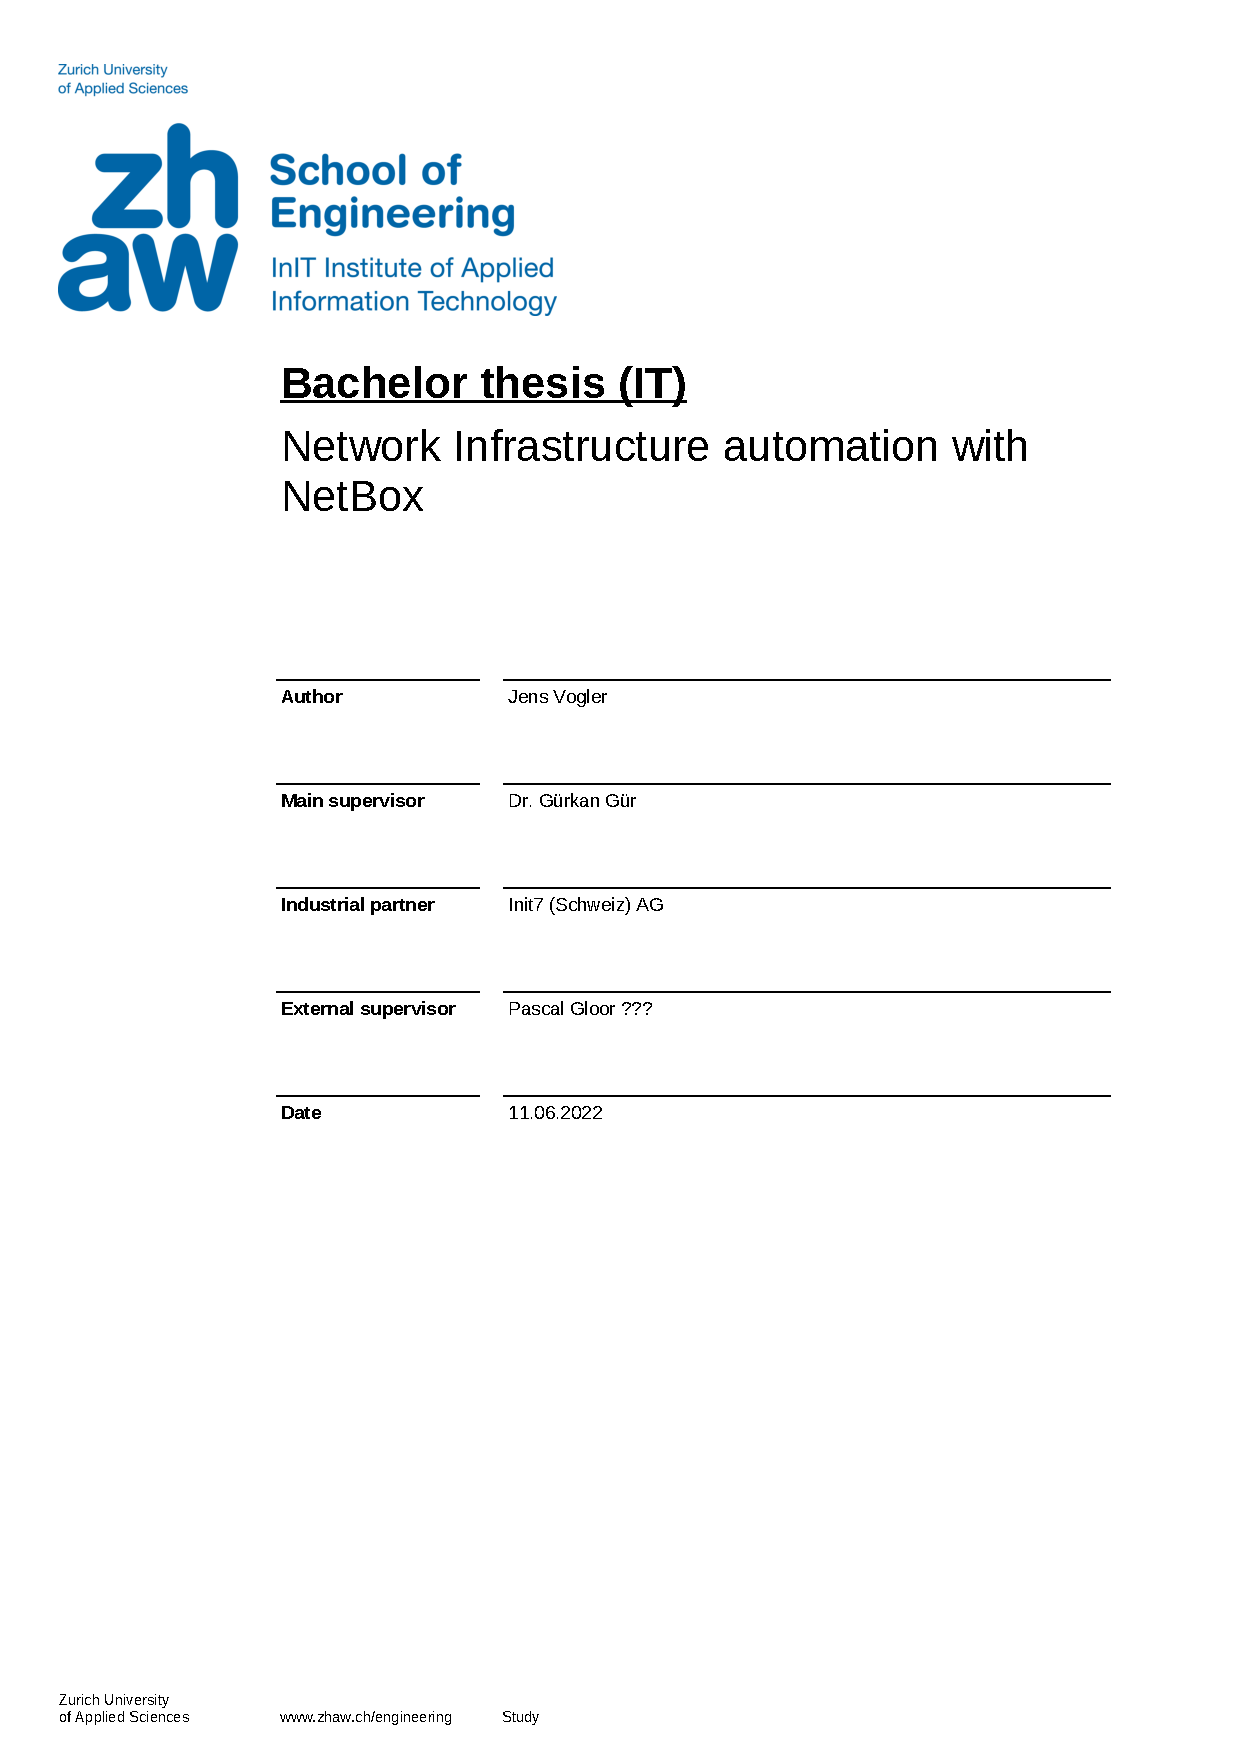
\includepdf[pages=-]{../Attachments/SoE-INIT_Bachelor-Titelblatt-Vorlage_en.pdf}
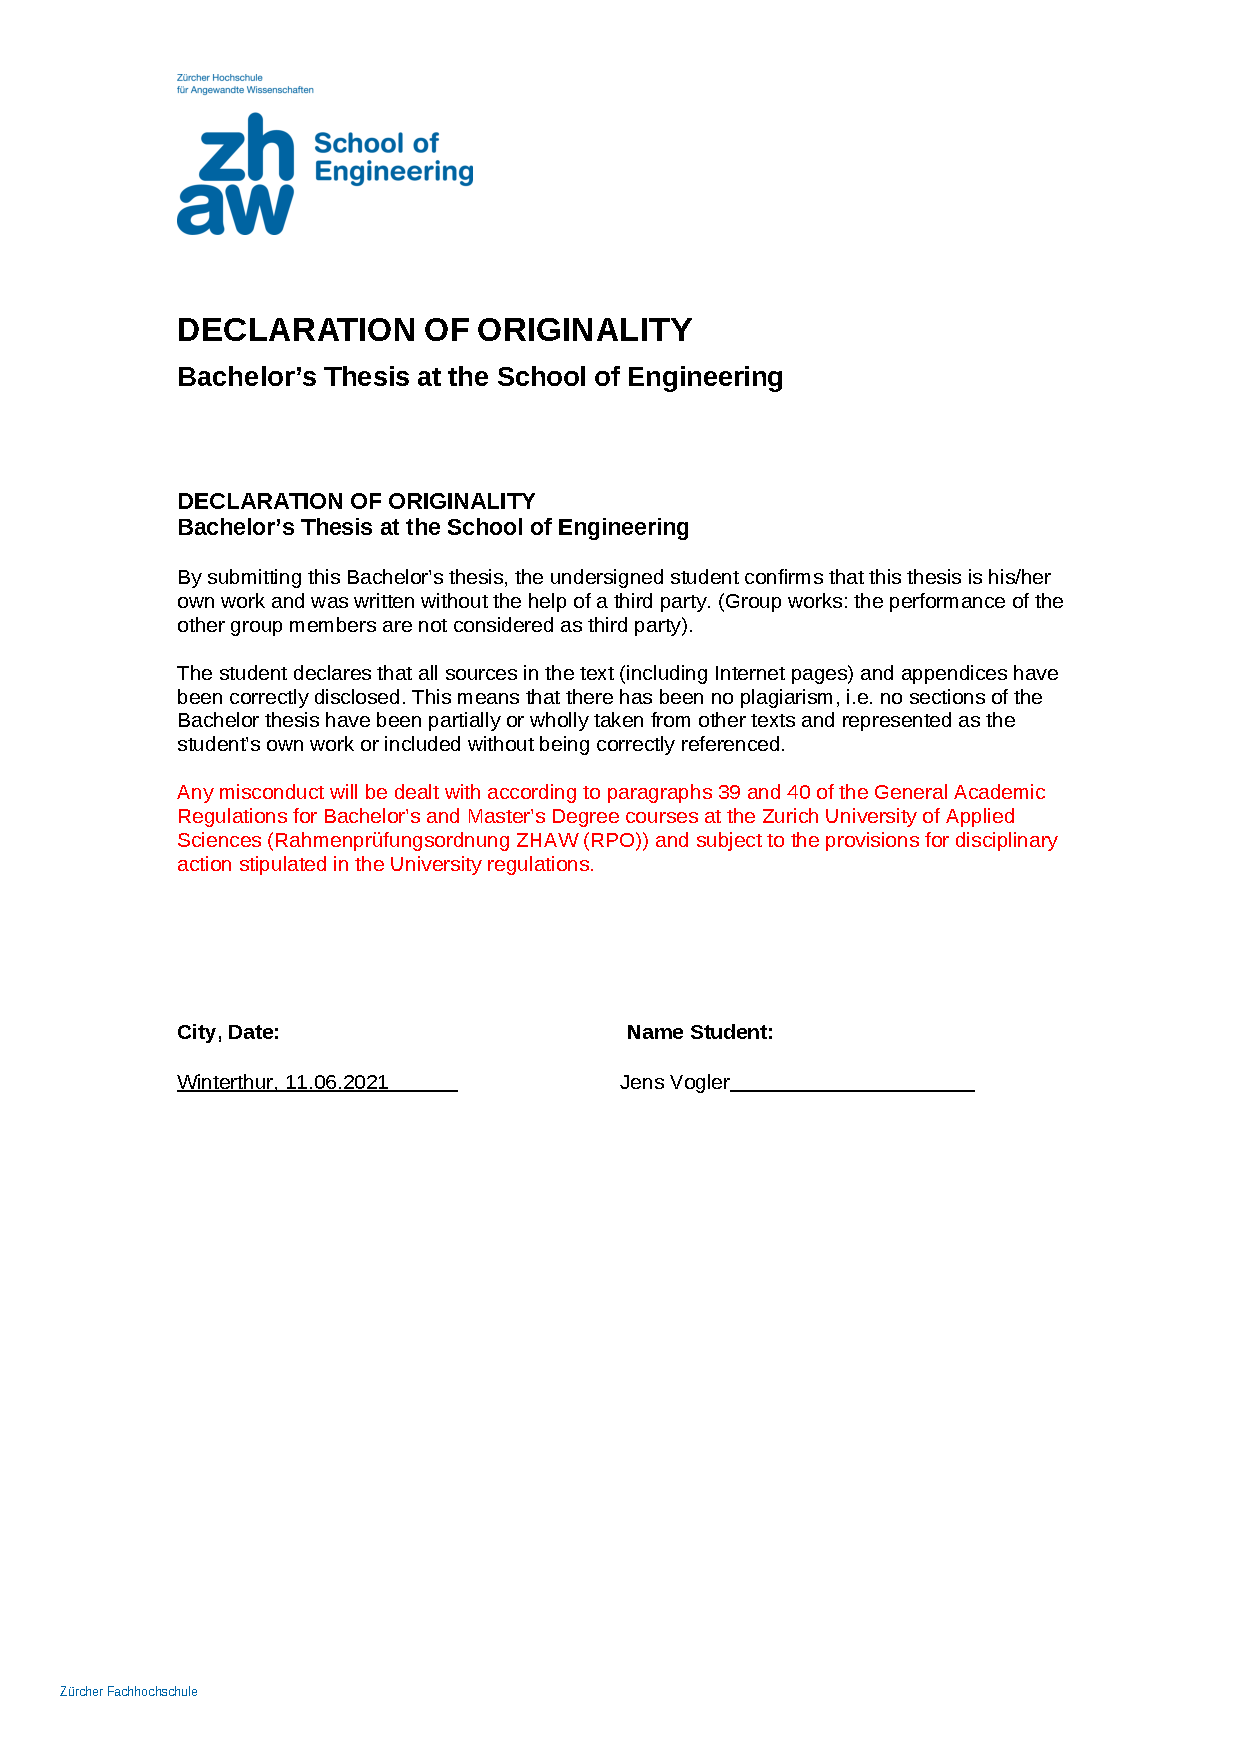
\includepdf[pages=-]{../Attachments/Erklaerung_BA_digital-_EN.pdf}


%** environments.tex: Predefined Environments
%****************************************************************************
%** Copyright 2002 by Lukas Ruf, ruf@topsy.net
%** Information is provided under the terms of the
%** GNU Free Documentation License http://www.gnu.org/copyleft/fdl.html
%** Fairness: Cite the source of information, visit http://www.topsy.net
%****************************************************************************

\newenvironment{sourcecode}%
{\vspace{0.5 cm} \footnotesize \verbatim}%
{\endverbatim \normalsize \vspace{0.5 cm}}

\newenvironment{inputverb}[1]%
{\vspace{0.5 cm} \footnotesize \verbatiminput{#1}}%
{\normalsize \vspace{0.5 cm}}

\newenvironment{inputverb_nospace}[1]%
{\footnotesize \verbatiminput{#1}}%
{\normalsize}


%% \newacronym{<id>}{<short>}{<long>}

%\newglossaryentry{glos:mpegts}{
% name=MPEG Transport Stream,
% description={Von der Moving Picture Experts Group entwickeltes Transportstream-Protokoll für Video/Audio-Übertragung}
%}

\newacronym{ISP}{ISP}{Internet Service Provider}
\newacronym{OSS}{OSS}{Operations Support System}
\newacronym{NMS}{NMS}{Network Management System}
\newacronym{BSS}{BSS}{Business Support System}
\newacronym{CPE}{CPE}{customer premises equipment}
\newacronym{ADSL}{ADSL}{asymmetric digital subscriber line}
\newacronym{DSL}{DSL}{digital subscriber line}
\newacronym{VDSL}{VDSL}{very high-speed digital subscriber line}
\newacronym{PoP}{PoP}{point of presence}
\newacronym{B2B}{B2B}{business to business}
\newacronym{BGP}{BGP}{Border Gateway Protocol}
\newacronym{MPLS}{MPLS}{Multiprotocol Label Switching}
\newacronym{OSPF}{OSPF}{Open Shortest Path First}
\newacronym{FTTH}{FTTH}{Fiber To The Home}
\newacronym{FTTS}{FTTS}{Fiber To The Street}
\newacronym{OTO}{OTO}{Optical Telecommunication Outlet}
\newacronym{IRM}{IRM}{infrastructure resource modeling}

\newacronym{OMDF}{OMDF}{Optical Main Distribution Frame}
\newacronym{CLI}{CLI}{command line interface}

\newacronym{OHDF}{OHDF}{Optical Handover Distribution Frame}
\newacronym{IGP}{IGP}{Interior gateway protocol}

%% TODO: Definition Network Element

\newglossaryentry{glos:snmp}{
    name=Sinmple Network Management Protocol,
    description={}
}



\newglossaryentry{glos:isp}{
 name=MPEG Transport Stream,
 description={Von der Moving Picture Experts Group entwickeltes Transportstream-Protokoll für Video/Audio-Übertragung}
}

%**Documentation****************

%** Zusammenfassung.tex
\clearpage
\null
\vfil % or it might be \null
\begin{center}\textbf{Abstract}\end{center}

Managing the configuration of network devices is a complex topic and relevant
to both small and large businesses. After identifying a lot of manual processes within Init7 AG,
an effort to find better solutions was started. There are a lot of different protocols and
software solutions attempting to solve this problem, but most of them are either
limited in functionality or are solutions by hardware vendors which only support
their own networking gear.
As Init7 is an open-source minded company, uses multiple vendors for their hardware
and needs such a solution, the idea started of creating a custom implementation
of a network management system. The goal was to utilize open source tooling
and create a system that focuses on being flexible and vendor-agnostic.
Init7 already uses NetBox, an open source DCIM/IPAM, for inventory and documentation purposes.
This sparked the idea to build a configuration management solution on top of NetBox.

Following the initial idea, a collaboration between ZHAW and Init7 was formed to
create a proof of concept within the scope of this thesis. Together with Init7
the goals were outlined, and a software project plan was created.

NETCONF/YANG was chosen as the method of configuration, as it provides a clean
interface for integration and is also supported by many major vendors.
Focus was also laid onto the security of the solution, as it needs to access
critical network infrastructure.

The resulting proof of concept, proved to be useful in real-world applications
within Init7 business use-cases. Two complete services were implemented and were
verified by the Init7 network engineering team. Since the project was a success,
there is a high chance that Init7 will continue work on this project to make it
ready for a production environment.

\clearpage
\null
\vfil % or it might be \null
\begin{center}\textbf{Zusammenfassung}\end{center}

Die Verwaltung der Konfiguration von Netzwerkgeräten ist ein komplexes 
Thema und relevant sowohl für kleine als auch für grosse Unternehmen. 
Nach der Identifizierung vieler manueller Prozesse innerhalb der Init7 AG, 
wurde ein Versuch gestartet, bessere Lösungen zu finden. Es gibt eine Vielzahl 
von Protokollen und Softwarelösungen, die versuchen, dieses Problem zu lösen, 
aber die meisten davon sind entweder aber die meisten von ihnen sind entweder 
in ihrer Funktionalität eingeschränkt oder sind Lösungen von Hardwareherstellern, 
die nur ihre eigenen Netzwerkgeräte unterstützen. ihre eigene Netzwerkausrüstung unterstützen.
Da Init7 ein Open-Source-Unternehmen ist, das seine Hardware von mehreren Anbietern 
bezieht und eine solche Lösung benötigt, entstand die Idee, eine eigene Implementierung 
eines Netzwerkmanagementsystems zu entwickeln. Das Ziel war es, Open-Source-Tools zu verwenden 
und ein System zu schaffen, das flexibel und herstellerunabhängig ist. Init7 verwendet bereits 
NetBox, ein Open Source DCIM/IPAM, für Inventarisierungs- und Dokumentationszwecke. 
Daraus entstand die Idee, eine Konfigurationsmanagementlösung auf der Grundlage von NetBox zu entwickeln.

Nach der ersten Idee kam es zu einer Zusammenarbeit zwischen der ZHAW und Init7, 
um im Rahmen dieser Arbeit einen Proof of Concept zu erstellen. 
Gemeinsam mit Init7 wurden die Ziele umrissen und ein Software-Projektplan erstellt.

Als Konfigurationsmethode wurde NETCONF/YANG gewählt, da es eine saubere Schnittstelle 
für die Integration bietet und zudem von vielen grossen Anbietern unterstützt wird. 
Ein weiterer Schwerpunkt lag auf der Sicherheit der Lösung, da sie auf kritische Netzwerkinfrastruktur
zugreifen muss. kritische Netzwerkinfrastruktur zugreifen muss.

Der daraus resultierende Konzeptnachweis erwies sich in realen Anwendungen als nützlich im Rahmen 
von Init7-Geschäftsanwendungen. Zwei vollständige Dienste wurden implementiert und wurden vom 
Init7-Netzwerktechnikteam verifiziert. Da das Projekt ein Erfolg war, besteht eine hohe Wahrscheinlichkeit, 
dass Init7 die Arbeit an diesem Projekt fortsetzen wird, um es für eine Produktionsumgebung bereit zu machen.


%** Vorwort.tex
\thispagestyle{empty}
\clearpage
\null
\vfil % or it might be \null
\begin{center}\textbf{Foreword}\end{center}

%** Table of Contents
\tableofcontents

%** Einleitung.tex: 
% - Nennt bestehende Arbeiten/Literatur zum Thema
% - Stand der Technik: Bisherige Lösungen des Problems und deren Grenzen
% - (Nennt kurz den Industriepartner und/oder weitere Kooperationspartner und dessen/deren Interesse am Thema Fragestellung)
% - Formuliert das Ziel der Arbeit
% - Verweist auf die offizielle Aufgabenstellung des/der Dozierenden im Anhang
% - (Pflichtenheft, Spezifikation)
% - Übersicht über die Arbeit: stellt die folgenden Teile der Arbeit kurz vor
% - (Angaben zum Zielpublikum: nennt das für die Arbeit vorausgesetzte Wissen)
% - (Terminologie: Definiert die in der Arbeit verwendeten Begriffe)
\chapter{\label{introduction}Introduction}
\thispagestyle{fancy}


\section{\label{introduction-current}State of current Technology}
% Describe current state of technology and solutions

Networking hardware makes out a huge part in our internet infrastructure. 
There is an increasing amount of hardware vendors varying in range of functionality. 
\glspl{ISP} are obvious customers of such hardware, but businesses of all sizes may have needs for all kinds of devices. 
This starts to pose the question, of how these devices shall be managed, especially when the need for scaling up arises. 
Many vendors supply configuration management solutions, also called \glspl{NMS} along their hardware offering, 
such as Cisco's ``Cisco DNA Center\cite{noauthor_cisco_nodate}'' or Juniper's ``Junos Space\cite{noauthor_junos_nodate}'' 
which might be the perfect fit in an environment wherein all hardware is obtained from the same vendor.
On the other hand, in mixed vendor environments, 
problems arise with these solutions as they primarily support their own hardware.

Since there's no ``one size fits all'' solution, one might want to come up with a custom solution.
In order to create a custom solution, one must know how devices are configured by \acrshort{NMS}s 
(or humans if that is automatable). There are numerous so-called network configuration protocols, 
such as \acrshort{SNMP}\cite{fedor_simple_1990}, CLI (e.g. via SSH or serial), NETCONF\cite{enns_network_2011} and others,
which can be used to remotely configure devices.

In order to configure devices, one must also know which devices exist within the infrastructure.
So called \acrfull{IRM} software is used to track the devices along with
information related to how they are connected and configured. 
While the above-mentioned \acrshort{NMS}'s usually provide such functionality, there are also
standalone solutions such as NetBox, which tracks everything from hardware to IP addresses.
Using the \acrshort{IRM} as the source of information, one would then be able to use a configuration protocol
to configure the devices according to one's needs.

\section{\label{introduction-goal}Goal / Aim}

% Describes the goal/aim of the work

The overarching goal is to provide a solution similar to an \acrshort{NMS} while utilizing open source
tools and software.
This will be achieved by extending NetBox with a plugin, which will allow an engineer to author configuration
templates which source their data from NetBox itself. 
These templates can then be applied to devices, wherein the plugin will generate the configuration and subsequently
apply it via a chosen configuration protocol.

As it is usually necessary to authenticate oneself in order to apply configuration to a device,
the issue of credential management and storage has to be solved.

\cn{Target open source space}
\cn{be vendor-agnostic}
\cn{compare transport protocols}
\cn{analyze compatibility}

% Separately describes the actual task to be performed, referencing the "Aufgabenstellung" of the BA



% Overview of the work

\section{\label{introduction-overview}Overview}



% Required knowledge for this paper



%** TheoretischeGrundlagen.tex:
\chapter{\label{theory}Theory}
\thispagestyle{fancy}


%** Vorgehen.tex:
% - Beschreibt die Grundüberlegungen der realisierten Lösung (Konstruktion/Entwurf) und die Realisierung als Simulation, als Prototyp oder als Software-Komponente etc.
% - (Definiert Messgrössen, beschreibt Mess- oder Versuchsaufbau, beschreibt und dokumentiert Durchführung der Messungen/Versuche)
% - (Experimente)
% - (Lösungsweg)
% - (Modell)
% - (Eingesetzte Software)
% - (Tests und Validierung)
\chapter{\label{methods}Methods}
\thispagestyle{fancy}

\section{Literature Research}

- Lots of papers on protocols
- Difficulty in finding concrete cases
- Lots of stuff is propiritary
  - Open Source solutions are very fragemented
  - Makes it hard to find examples for working solutions

\section{Software Engineering Method}

\section{Evalution Method}



%** Resultate.tex:
% - Zusammenfassung der Resultate
\chapter{\label{results}Results}
\thispagestyle{fancy}

\section{Requirements Analysis}

The first step of the development process was to find out and define
how the solution should work. In collaboration with the Init7 network
engineering team, the core use cases were defined. As this was only
a proof of concept, the use cases were only described in a brief and
concise format. Furthermore, a consensus was formed how an engineer
should be able to operate with the plugin in general.

The following use cases were defined based on the design idea that
the engineer is able to write configuration templates which utilize data
available in NetBox, which subsequently can be deployed to a device.

\begin{enumerate}[label=U.\arabic*]
  \item{\label{uc-agg}} \textbf{Data Aggregation} 
  The engineer is able to easily configure and discover the available
  context information for authoring a template.
  \item{\label{uc-tmpl}} \textbf{Template Authoring}
  A view with an editor exists to author configuration templates.
  This view also provides a preview of the context data and this data
  can be used to preview the rendered template.
  \item{\label{uc-appl}} \textbf{Configuration Deployment}
  The engineer is able to apply a previously configured template
  to a network device.
  \item{\label{uc-cred}} \textbf{Credential Management}
  An authorized engineer is able to configure credentials which are used
  in the configuration deployment. The usage access to these credentials must
  be restrictable to specific users or groups. The ability to modify these
  credentials must also be restrictable to specific users or groups.
\end{enumerate}

In addition to the use cases, a decision has to be made on which
configuration method is used. In order to do this, the following compatibility
matrix was created:

\begin{center}
\begin{tabular}{l|c|c|c|c}
  Vendor & CLI & SNMP & NETCONF/YANG & HTTP API \\
  \hline\hline
  Cisco & Yes & Yes & Yes & No \\
  \hline
  MikroTik & Yes & No\textsuperscript{1} & No & Yes \\
  \hline
  Juniper & Yes & Yes & Yes & Yes \\
  \hline
  Extreme Networks & Yes & Yes & Yes & Yes \\
  \hline
  FS & Yes & No\textsuperscript{1} & Yes & Yes \\
  \hline
  Nokia & Yes & N/A & Yes & N/A \\
  \hline
  Ubiquity & Yes & No\textsuperscript{1} & No & Yes \\
\end{tabular}
\end{center}

\textsuperscript{1} SNMP is supported, but only supports read
operations, which makes it unsuitable for configuration deployment.

The above list of vendors include both vendors which are used within Init7
and other vendors which often appear in enterprise and ``power user''
environments. (Basic consumer hardware was disregarded since they usually
do not provide any standardized way to configure them.)

\paragraph{Configuration method decision} The HTTP APIs were excluded first
from the selection, since after some research, it became clear that they
differ wildly between vendors which makes it near impossible to write
a generic solution for. SNMP was excluded for both its age and lack
of write support in many vendor implementations. In the end, NETCONF/YANG was
chosen over the CLI because of the benefit of the model driven configuration
outlined in \ref{theory:conf:yang}.

\section{Application structure / Architecture}

To bridge the gap between the inventory management provided by NetBox and communicating with the actual hardware,
the solution is divided into layers.
In order to facilitate authentication and authorization there is the ``Credential Access Manager'' which communicates
with an external credential store. The access manager provides a user interface to enter and manage credentials, as well
as restricting who has access to these credentials by integrating into the NetBox permission system.
The ``Device Context Provider'' enables a user to define what information for a specific device shall be pulled.
Using the existing GraphQL API provided by NetBox, the user can easily identify what information is available and how it is
accessed. After the context data is defined it will subsequently be used in the ``Configuration Template Editor''
where the user writes a template using the previously defined context data. This template can then be applied to
a class of devices utilizing constraints such as tags or locations.
Lastly, the ``Configuration Transport'' module pulls the configuration template and the credentials for a specific device
and pushes it to the actual device.


\begin{figure}[h]
  \centering
  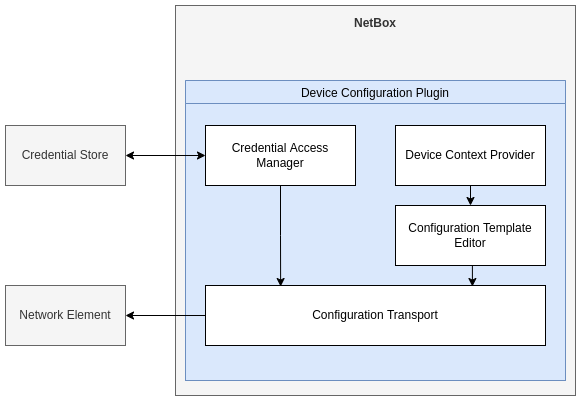
\includegraphics[width=0.8\textwidth]{Software-Arch}
  \caption{Software Architecture Concept}
  \label{fig:soft-arch}
\end{figure}



\subsection{Credential Access Manager}

In order to offload parts of the potential security issues with storing
credentials, an external credential manager is used.
In this case, HashiCorp Vault is used, as it is relatively easy to
set up and became one of the de facto solutions in multiservice
environments. To integrate Vault into the NetBox plugin, the client
library \icode{hvac} is used. A small abstraction layer is built
on top of the library, to make it easy for the rest of the plugin
to store and retrieve secrets.

\subsection{Device Context Provider}

Rendering templates in general usually requires some sort of context data
(i.e. a template for a marketing mail might require the customers name.)
NetBox already has a functionality called ``Export Templates'' which
allow a user to write templates to export lists of data with a custom
output format. What makes these ``Export Templates'' hard to use is that
they utilize the python objects mapped from the database as context,
which makes it somewhat necessary to know the internals of NetBox to
use them effectively.

Though what NetBox also provides, is a GraphQL API. GraphQL allows
the API consumer to specify exactly what data one is interested in,
in addition to requiring a complete specification for the API.
Using this specification, one can use a client like ``GraphiQL'',
which provides the user with autocompletion and documentation
access. As this client is built-in to NetBox, it provides an
intuitive user interface for specifying context data.

The Device Context Provider is therefore implemented by accepting
GraphQL queries in its configuration, which the user can author
with ``GraphiQL''.

\subsection{Configuration Template Editor}

Since the template the user writes should result in a valid NETCONF RPC
message, which is constructed using XML syntax, a code editor like experience
is preferred. Since NetBox is a browser based application, JavaScript based
code editors were evaluated and the Ace editor was chosen based on its
lightweightness and simplicity.

The template editor is split into three panes, where the engineer can see
the context data, the template content and a preview. This way, the engineer
is always aware what context data he can use, and can quickly see what the result
of a rendered template looks like.

\subsection{Configuration Transport}

Lastly, the configuration transport component ties all the other components
together and enables the deployment of a configuration to a device.
The actual deployment is implemented through the \icode{ncclient} library,
which manages the NETCONF connection and supplies an interface to send
RPCs through it.

Additionally, the ``glue'' is implemented to facilitate the rendering of
the template, retrieving the credentials and subsequently deploying the
configuration.
Special care needs to be taken when retrieving the credentials, as the
configured authorization needs to be enforced to prevent users from
deploying configuration when they are not allowed to do so.


\section{\label{eval-security}Security Evaluation}

To evaluate the security of the implemented solution, scenarios based on
the threat actors defined in \ref{method:eval-sec} were drawn up and
subsequently checked.


\begin{enumerate}[label=S.\arabic*]
  \item An {\it external actor} only with the knowledge
  that the system exists, cannot gain any form of access to the system or infrastructure. \\
  NetBox is behind a firewall which only allows access from within the company network.
  Additionally, NetBox is protected with standard username and password authentication,
  which has currently no known exploits for the latest version of Django (the web framework NetBox is based on).
  The impact is therefore negligible.

  \item An {\it external actor} gains non-elevated privileges to the server NetBox is running on. \\
  In a standard NetBox deployment, the instance is running as a separate user or even within a container.
  Low privilege access on Linux inspect memory of other processes, therefore the stored credentials
  cannot be extracted. If the actor has access to the configuration files, he may be able to discover the credentials of the
  database NetBox uses. In that case, the actor may be able to create a user within NetBox and gain administrative access
  to the running instance. While the actor is now able to deploy configurations to devices using the existing credentials,
  the credentials themselves cannot be extracted, as the secret, once stored, is never revealed to any user ever again.
  The privilege escalation within NetBox can be prevented through proper access restrictions to both the database
  and configuration data.
  The impact is high, but with proper configuration it can be significantly reduced.

  \item An {\it unauthorized employee} without any explicit privileges attempts to deploy a configuration to a device. \\
  The employee is not able to trigger a deployment because of the authorization check at the credential access manager.
  But, the employee is able to modify configuration templates, potentially tricking an authorized user to deploy it to a device.
  This is something that was missed during development and must be fixed before usage in production.

  \item An {\it unauthorized employee} with only usage access on specific credentials attempts to change the authentication information,
  potentially causing a denial of service for the operation of the configuration management. \\
  This is prevented through the authorization check in the credential access manager. The main risk is misconfiguration within the
  credential access manager if too permissive privileges are set.

\end{enumerate}

\section{Scenario Evaluation}

The following sections describe two chosen real-world scenarios within Init7.
More specifically, they are services which can be ordered by customers and also
require some manual work by network engineers in the current process.

The goal is to show how manual labor can be replaced or supported by the
created NetBox plugin.

\subsection{Fiber7}

Fiber7 is Init7's flag-ship product in the private consumer space,
providing consumers a \acrshort{P2P} fiber-optical connection directly into
Init7 infrastructure. Since this is the most commonly sold product by Init7
it is already one of the most streamlined processes throughout the department
with work being largely automated.

\begin{figure}[h]
  \centering
  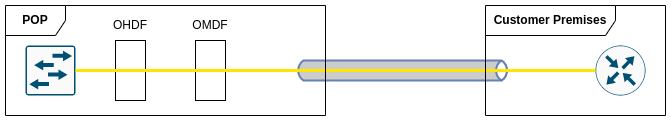
\includegraphics[width=\textwidth]{P-Fiber7}
  \caption{Fiber7 Service Diagram}
  \label{fig:fiber7}
\end{figure}

When the work-order arrives at the network engineer, it has already been decided
or defined at which \acrshort{POP}, network switch and interface the customer
will be connected to. The engineer will then go through the following process:

\begin{enumerate}
  \item A new service configuration ticket arrives
  \item Verify that there is no other active use on the chosen interface
  \item Apply the default configuration profile for Fiber7 private customers on the interface
  \item If the customer requested a static IP address, configure it on the DHCP server
  \item If the customer requested a prefix, configure it on the router connected to the switch
  \item If the customer does not specify a specific service activation date, enable the switchport
  \item Update NetBox with the performed configuration
  \item Update the service configuration ticket
\end{enumerate}

While the process might have seven steps, usually not all of that work is required.
When choosing the interface for the new service, it is verified through the \acrshort{OSS}
that the port has no other active use.
Interfaces have the Fiber7 private customer profile configured by default
if it was previously unused or was previously used for the same service,
rendering step 3 usually unnecessary.
Most commonly, customers do not request static IP addresses or prefixes as
they are an additional cost to the subscription and are only used by ``power-users'',
rendering steps 4 and 5 unnecessary.

The key observation that can be made, is that there are multiple manual steps
which can be prone to mistakes, yet they are always performed the same way. This makes
them good candidates for automation. Thus, the goal is to restructure the process
to the following:

\begin{enumerate}
  \item A new service configuration ticket arrives
  \item Within NetBox:
  \begin{enumerate}
    \item Set the service field on the interface to Fiber7
    \item 
  \end{enumerate}
\end{enumerate}

\cn{(above) list not complete}

\cn{Describe process to extract template information}

\cn{Describe verification}

\subsection{Business Optical Service}


\begin{figure}[h]
  \centering
  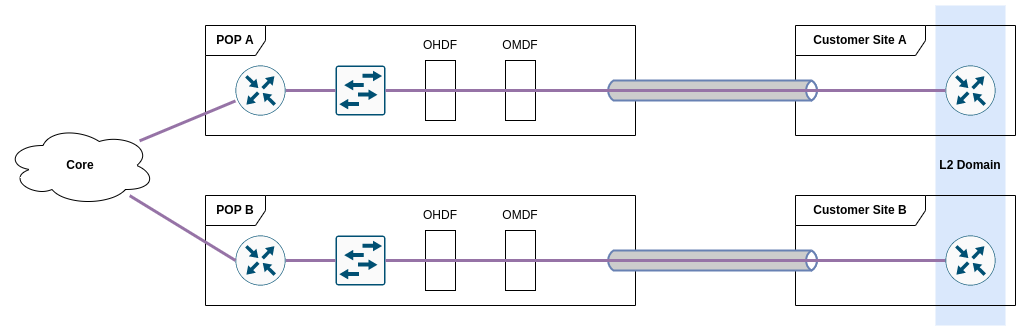
\includegraphics[width=\textwidth]{P-S2S}
  \caption{Business Optical Service Diagram}
  \label{fig:s2s}
\end{figure}

\cn{
 - B2B customer (standard)
  - Access Port with less configuration  \\
  - VLAN 600  \\
  - Static IP on router  \\
  - Static Route on router  \\
 - B2B customer (new)  \\
  - Trunk Port  \\
  - Allowed VLAN 600  \\
  - + same as standard?  \\
 - B2B Site-2-Site  \\
  - VLL through MPLS  \\

 - MikroTik ZTE  \\
 }

%** DiskussionAusblick.tex:
% - Bespricht die erzielten Ergebnisse bezüglich ihrer Erwartbarkeit, Aussagekraft und Relevanz
% - Interpretation und Validierung der Resultate
% - Rückblick auf Aufgabenstellung, erreicht bzw. nicht erreicht
% - Legt dar, wie an die Resultate (konkret vom Industriepartner oder weiteren Forschungsarbeiten; allgemein) angeschlossen werden kann; legt dar, welche Chancen die Resultate bieten.
\chapter{\label{discussion}Discussion}
\thispagestyle{fancy}

\section{Achieved goals}

To summarize, the goals of providing a flexible and vendor-agnostic configuration was reached
partially. For a proof of concept work being able to model
real world offerings which are high in complexity, and subsequently configure them correctly,
proves that combining NetBox with NETCONF can create a powerful \acrshort{OSS}.

While it was verified that quite a few other vendors support NETCONF as well, no concrete
testing could be performed due to time and also equipment constraints.

After working with together with the Init7 engineering staff and later also presenting
the finished product, the consensus was to pursue this avenue further. As the project
is open source, this may also bring future benefits to the general networking community.

Some flaws were found in the security of the work, which have to be addressed before
it is used in a production environment. While one could describe the finding as an
oversight, a security audit may be necessary in order to ensure that no other
oversights were missed, especially for such a sensitive system.

\section{Problems during development}

Major time blockers were inconsistencies especially with Cisco's IOS-XE software.
Several bugs in their NETCONF implementation were identified, such as sections of configuration
entirely missing from the YANG models, \icode{<get-config>} operations not returning the full data,
and even \icode{<edit-config>} nodes which are documented in the YANG model but proved to be non-functional
in practice. Several support tickets were opened with Cisco, without response yet.



%** Verzeichnisse.tex:
\chapter{\label{references}References}
\thispagestyle{fancy}

\raggedright
\printbibliography[title={Bibiliogrpahy},heading=subbibnumbered]
% [title={Literaturverzeichnis},heading=subbibnumbered] würde nummerieren

\pagebreak
\printglossary

%** Table of Figures
\pagebreak
\listoffigures

\pagebreak
\printglossary[type=\acronymtype]

%** Anhang.tex:

\chapter{\label{appendix}Appendix}
\thispagestyle{fancy}

%** end the document environment
\end{document}
